\section{Refactoring} \label{sec:s4_refactoring}
%%% Intro paragraph --> Why do we refactor?

%%% How do we refactor?

%%% Summary --> Did the refactoring give us the desired results?

\subsection{class architecture}
In order to fully describe the system design of the hotMap server, the UML v2.5 standard are used to express how the class hierarchy were implemented. UML is a well known modeling language, for visualizing software system designs in order to more easily describe the static structure of a software system.
Therefor a UML class diagram are used for describing the model layer of the hotMap server.
The UML v2.5 standard for class diagram are mainly used for modeling the class diagram, but scala has some features such as mixin which cannot be fully represented using the UML standard alone.

Mixin is an language dependent functionality, which allows a class $A$ to contain methods from other classes or interfaces without having that $A$ is a generalization of these other classes or traits. How class $A$ gain access to those methods through mixin are defined by the language. Mixin avoids inheritance ambiguity such as the diamond problem while having the ability to extend multiple classes, because it's not possible to inherit from a mixin type.

Scala does not have interfaces, but instead uses traits. These are similar but allow for default implementation of methods within the trait. When a concrete classes extends traits, it is called a realization of that trait, which in UML are indicated by a dashed arrow from the class to the interfaces. In scala traits can also be instantiated if all it's instance variables and methods are implemented. In scala only traits can be mixed into classes or another trait, but not the other way around.

In scala type aliases of mixin types are used to denoted a class mixed with some other class. As an example of this we have on \cref{fig:class} that $Point$ is a alias for any type which realizes $Coordinate$ mixed with a $Weight$. As mentioned before UML cannot represent mixin, so it was chosen to show this by drawing a realization arrow with a mixin stereotype from the alias to the mixed type. Stereotypes are denoted by some text surrounded with $<<$ and $>>$ above the arrow.

\begin{figure}[!htb]
\centering
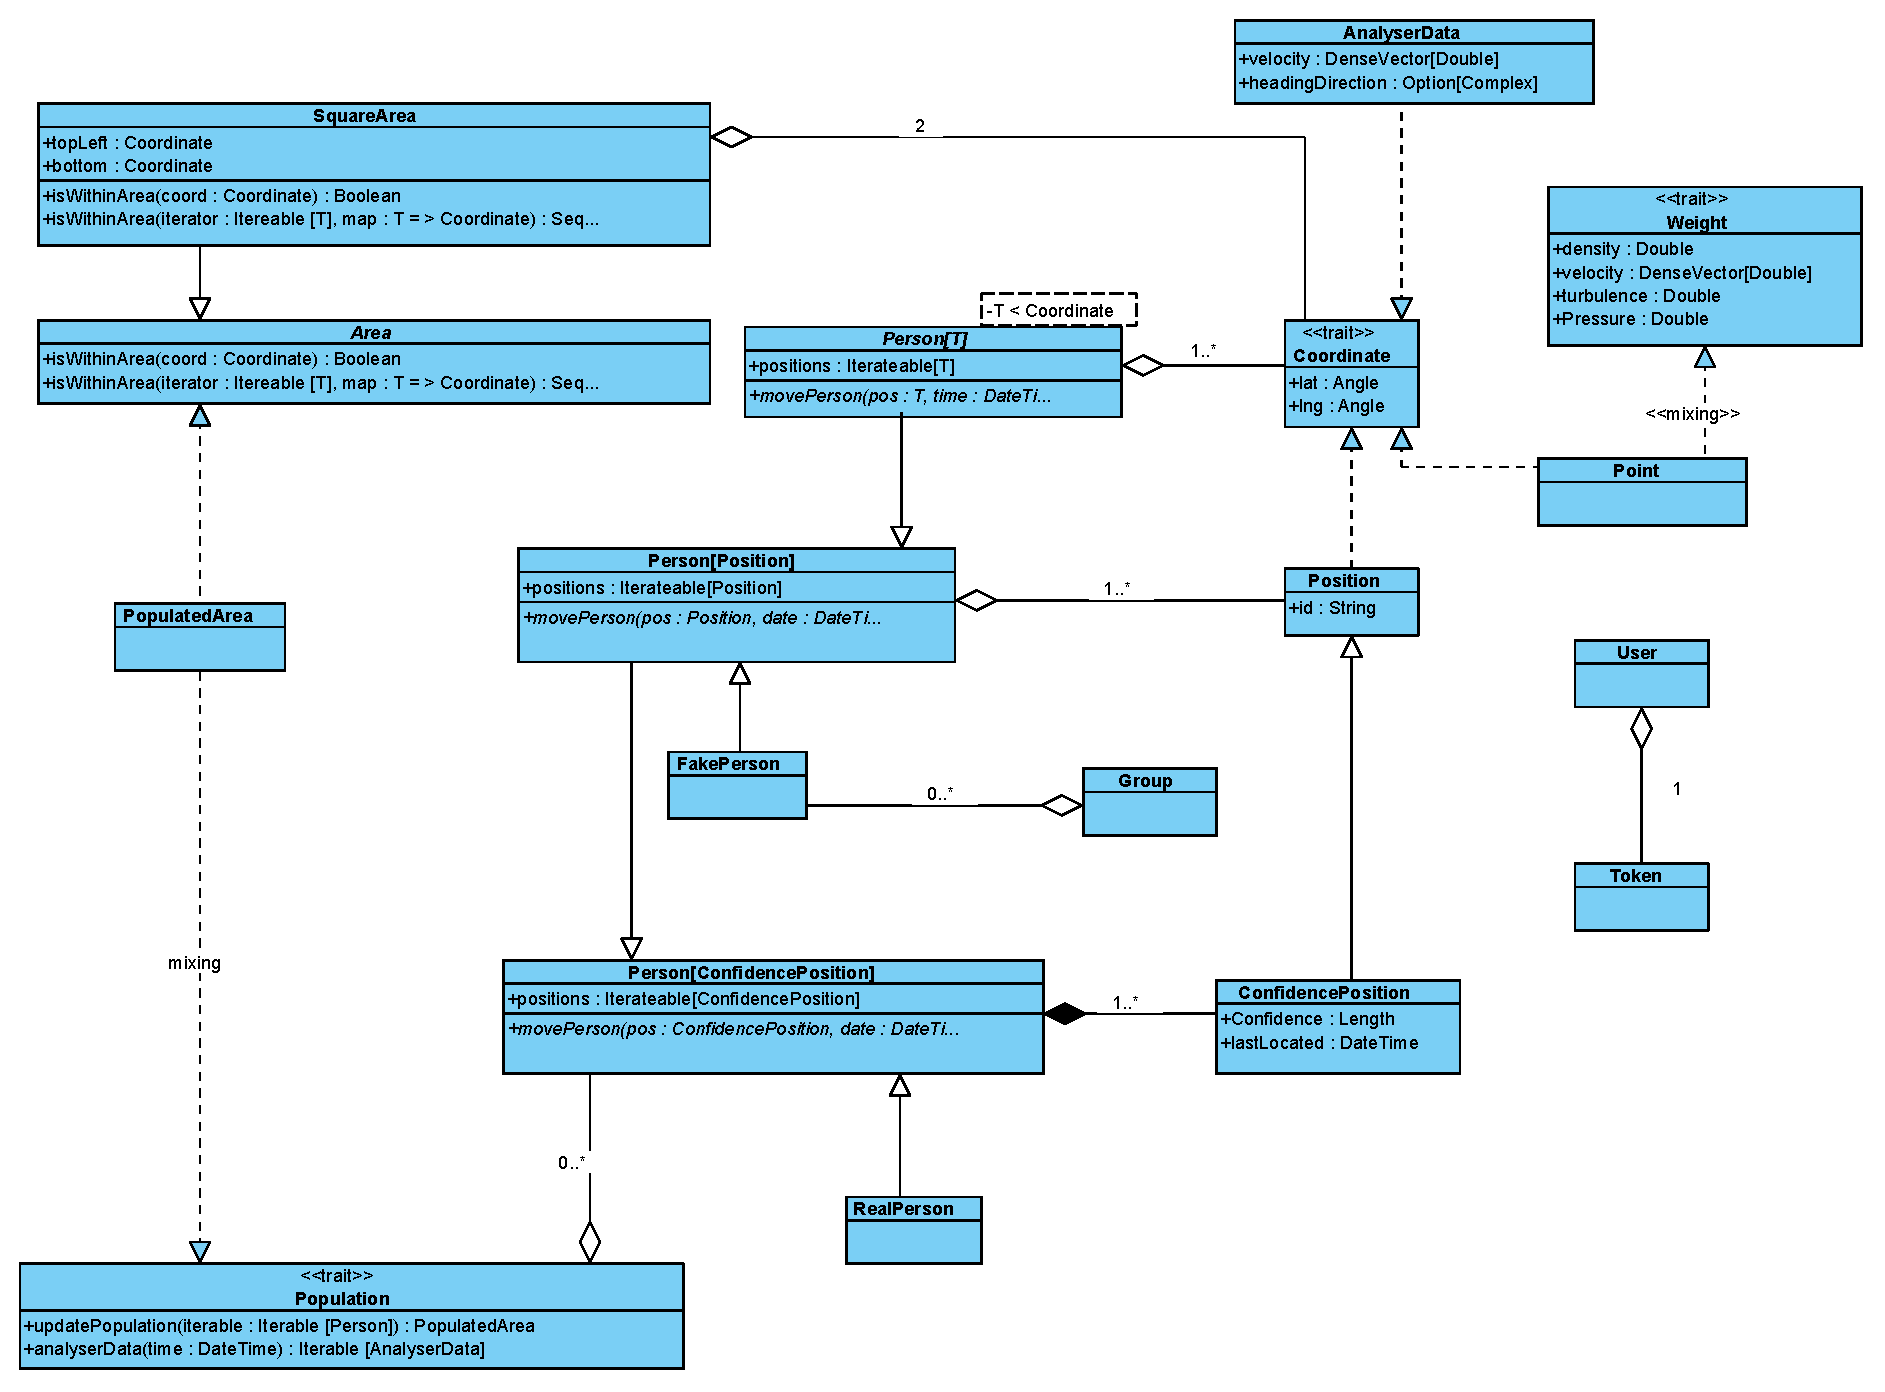
\includegraphics[scale=.7]{figures/class.eps}
\caption{Digraph.}
\label{fig:class}
\end{figure}
